\documentclass[10pt,landscape]{article}
\usepackage{multicol}
\usepackage{calc}
\usepackage{ifthen}
\usepackage[landscape]{geometry}
\usepackage{hyperref}
\usepackage{float}

\usepackage{tikz}
\usepackage{amsmath}
\usetikzlibrary{arrows}
\usepackage{float}
\usetikzlibrary{shapes}
\usetikzlibrary{intersections}
\usepackage{circuitikz}
\usepackage{pgfplots}
\pgfplotsset{compat=1.13}
\usepackage{graphicx}
\usepackage{trfsigns}
\usepackage{array}

\newcommand*\circled[1]{\tikz[baseline=(char.base)]{
            \node[shape=circle,draw,inner sep=2pt] (char) {#1};}}

% This sets page margins to .5 inch if using letter paper, and to 1cm
% if using A4 paper. (This probably isn't strictly necessary.)
% If using another size paper, use default 1cm margins.
\ifthenelse{\lengthtest { \paperwidth = 11in}}
	{ \geometry{top=.5in,left=.5in,right=.5in,bottom=.5in} }
	{\ifthenelse{ \lengthtest{ \paperwidth = 297mm}}
		{\geometry{top=1cm,left=1cm,right=1cm,bottom=1cm} }
		{\geometry{top=1cm,left=1cm,right=1cm,bottom=1cm} }
	}

% Turn off header and footer
\pagestyle{empty}

\def\arraystretch{5}
 

% Redefine section commands to use less space
\makeatletter
\renewcommand{\section}{\@startsection{section}{1}{0mm}%
                                {-1ex plus -.5ex minus -.2ex}%
                                {0.5ex plus .2ex}%x
                                {\normalfont\large\bfseries}}
\renewcommand{\subsection}{\@startsection{subsection}{2}{0mm}%
                                {-1explus -.5ex minus -.2ex}%
                                {0.5ex plus .2ex}%
                                {\normalfont\normalsize\bfseries}}
\renewcommand{\subsubsection}{\@startsection{subsubsection}{3}{0mm}%
                                {-1ex plus -.5ex minus -.2ex}%
                                {1ex plus .2ex}%
                                {\normalfont\small\bfseries}}
\makeatother

% Define BibTeX command
\def\BibTeX{{\rm B\kern-.05em{\sc i\kern-.025em b}\kern-.08em
    T\kern-.1667em\lower.7ex\hbox{E}\kern-.125emX}}

% Don't print section numbers
\setcounter{secnumdepth}{0}


\setlength{\parindent}{0pt}
\setlength{\parskip}{0pt plus 0.5ex}


% -----------------------------------------------------------------------

\begin{document}

\raggedright
\footnotesize
\begin{multicols}{2}

% multicol parameters
% These lengths are set only within the two main columns
%\setlength{\columnseprule}{0.25pt}
\setlength{\premulticols}{1pt}
\setlength{\postmulticols}{1pt}
\setlength{\multicolsep}{1pt}
\setlength{\columnsep}{2pt}

\section{Data Conversion Chain | 20-02-2017}

\begin{figure}[H]
    \begin{center}
        \tikzset{font={\fontsize{8pt}{12}\selectfont}}
        \begin{circuitikz}[x=0.021\linewidth,y=0.021\linewidth]

        \draw[name path=chain]
           (0,0) node[above]{$V_{in}$} to[short,o-] ++(0.2, 0)
           to[lowpass,->] ++(6,0)
           to[twoport,t=S\&H,n=nsh] ++(6,0)
           to[adc,n=nad] ++(6,0)
           to[dsp] ++(6,0)
           to[dac,n=nda] ++(6,0)
           to[lowpass,n=nlp] ++(6,0)
           to[short,-o] ++(0.2,0) node[above]{$V_{out}$};

        \path[name path=labels]
           (0,-10) -- ++(3.2, 0) node[draw,shape=circle]{5}
           -- ++(6,0) node[draw,shape=circle]{4}
           -- ++(6,0) node[draw,shape=circle]{3}
           -- ++(6,0) node[draw,shape=circle]{1}
           -- ++(6,0) node[draw,shape=circle]{2}
           -- ++(6,0) node[draw,shape=circle]{6}
           -- ++(6,0);

        \draw[name path=sndr]
        (36.4,-0.5) to[short] ++(0, -0.5)
        to[short] ++(3, 0)
        to[short] ++(0,-4) node[draw,below]{SNDR}
        ++(0, -3) node[align=center]{signal to noise \\ and distortion ratio};

        \draw[name path=cd,dashed] (9.2,-6) node[above,rotate=90]{continuous} node[below,rotate=90]{discrete}
        -- (nsh.south) (nsh.north) -- (9.2,6) node{};

        \draw[name path=ad,dashed] (15.2,-6) node[above,rotate=90]{analog} node[below,rotate=90]{digital}
        -- (nad.south) (nad.north) -- (15.2,6) node{};

        \draw[name path=da,dashed] (27.2,-6) node[above,rotate=90]{digital} node[below,rotate=90]{analog}
        -- (nda.south) (nda.north) -- (27.2,6) node{};

        \draw[name path=lp,dashed] (33.2,-6) node[above,rotate=90]{discrete} node[below,rotate=90]{continuous}
        -- (nlp.south) (nlp.north) -- (33.2,6) node{};

        \end{circuitikz}
    \end{center}
    \caption{A typical signal chain}
    \label{fig:chain}
\end{figure}

\subsubsection[chain1DSP]{\circled{1} DSP}
The equivalent ouput voltage can be expressed with \ref{eq:eq_vtg}. It's maximum can be described with \ref{eq:eq_vtg_max}
\begin{equation}
    V_{eq} = V_{ref} \Big(\sum^N_{i=1}b_i 2^{-i}\Big)
    \label{eq:eq_vtg}
\end{equation}
\begin{equation}
    V_{eq} = V_{ref}\Big(1 - 2^{-N}\Big)
    \label{eq:eq_vtg_max}
\end{equation}

This is a representation in UINT. In most realworld impelemntations INT using 2's complement is required. Sometimes if there is peak currents, Gray-Code is to be used to minimize peak currents!

The quantizer-error is defined with equation \ref{eq:quantizer_err}.

\begin{equation}
    V_{e} = V_{in} - V_{eq}
    \label{eq:quantizer_err}
\end{equation}

It is assumed that the error behaves like white noise\footnote{White noise means that the noise has the same amplitude for every frequency.} because the digital signal is a sequence of pulses. If this is fourier transformed a constant spectral density is received.

\begin{figure}[H]
    \begin{align*}
        \centering
        \begin{tikzpicture}[baseline,declare function={unipdf(\x,\xl,\xu)=(\x>\xl)*(\x<\xu)*1/(\xu-\xl);}]
            \begin{axis}[
                anchor=center,
                width=0.5\linewidth,
                samples=100,
                const plot mark mid,
                scaled ticks = false,
                ymin=0,ymax=0.5,
                xmin=-3,xmax=3,
                xtick={0},
                ytick={0}]
                \addplot [orange] {unipdf(x,-5,5)};
            \end{axis}
        \end{tikzpicture}
        \text{ }&\overset{\mathcal{F}}{\Laplace}\text{ }\delta(t) \\
        \text{spectral density }&\overset{\mathcal{F}}{\Laplace}\text{ autocorrelation function}
    \end{align*}
\end{figure}

Since the quantizer error has the probability density function of white noise, it can be depicted with the function seen in \ref{fig:prob_dens_func_quantizer}.

\begin{figure}[H]
    \centering
    \begin{tikzpicture}[declare function={unipdf(\x,\xl,\xu)= (\x>\xl)*(\x<\xu)*1/(\xu-\xl);},x=0.021\linewidth,y=0.021\linewidth]
        \begin{axis}[
            samples=100,
            const plot mark mid,
            scaled ticks = false,
            ymin=0,ymax=0.5,
            xmin=-3,xmax=3,
            xtick={-2,0,2},
            xticklabels={-$\frac{LSB}{2}$,0,$\frac{LSB}{2}$},
            xlabel={$V_e$},
            ytick={0.25},
            yticklabels={$\frac{1}{LSB}$},
            ylabel={$\rho(V_e)$}]
            \addplot [orange] {unipdf(x,-2,2)};
        \end{axis}
    \end{tikzpicture}
    \caption{Probability density function of the quatizer error}
    \label{fig:prob_dens_func_quantizer}
\end{figure}

With the knowledge of the fact that the variance equals the RMS\footnote{root mean square} value, depicted in equation \ref{eq:rms_variance} and thus \ref{eq:variance_quantizer_err}, we can now find the SNR\footnote{signal to noise ratio} value with solving equation \ref{eq:snr_base}

\begin{equation}
    (rms)^2 = \sigma,\text{ $\sigma$ is the standard deviation}
    \label{eq:rms_variance}
\end{equation}

\begin{align}
    \sigma_e^2 &= \int_{-\infty}^{+\infty}V_e^2\rho(V_e)dV_e \\
    &= \int_{-\frac{LSB}{2}}^{+\frac{LSB}{2}}\frac{V_e^2}{LSB}dV_e \\
    &= \frac{1}{LSB}\frac{1}{3}V_e^3\Big|_{-\frac{LSB}{2}}^{+\frac{LSB}{2}} \\
    &= \frac{LSB^2}{12} = \frac{1}{12}V_{ref}^22^{-2N}
    \label{eq:variance_quantizer_err}
\end{align}

\begin{align}
    SNR &= \frac{V_{sig, rms}^2}{V_{n, rms}^2} \\
    &= \frac{\Big(\frac{V_ref}{2}\frac{1}{\sqrt{2}}\Big)^2}{\frac{1}{12}V_{ref}^22^{-2N}} \\
    &= N\cdot 6.02dB + 1.76dB
    \label{eq:snr_base}
\end{align}

Using this equation a statement about the ENOB\footnote{effective number of bits} can be made, having a look at the SNR equation optained. This is given in \ref{eq:neff}.

\begin{equation}
    N_{eff} = ENOB = \frac{SNDR - 1.76dB}{6.02dB}
    \label{eq:neff}
\end{equation}

\subsubsection[chain2DA]{\circled{2} D/A}

\begin{figure}[H]
    \centering
    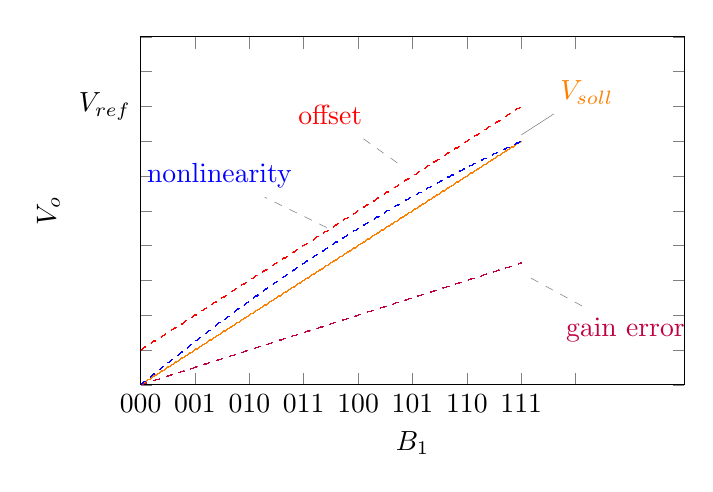
\begin{tikzpicture}[declare function={unipdf(\x,\m,\q)=(\m*\x+\q);},x=0.021\linewidth,y=0.021\linewidth]
        \begin{axis}[
            height=6cm,
            width=0.7\columnwidth,
            samples=300,
            const plot mark mid,
            scaled ticks = false,
            ymin=0,ymax=10,
            xmin=0,xmax=10,
            xtick={0,1,2,3,4,5,6,7,8},
            xticklabels={000,001,010,011,100,101,110,111},
            xlabel={$B_1$},
            ytick={0,1,2,3,4,5,6,7,8,9,10},
            yticklabels={,,,,,,,,$V_{ref}$},
            ylabel={$V_o$}]
            \addplot [orange][domain=0:7]{unipdf(x,1,0)} node[left,pos=1,pin=35:{$V_{soll}$}] {};
            \addplot [dashed,red][domain=0:7]{unipdf(x,1,1)} node[above,pos=0.7,pin=135:{offset}] {};
            \addplot [dashed,purple][domain=0:7]{unipdf(x,0.5,0)} node[below,pos=1,pin=-45:{gain error}] {};
            \addplot [dashed,blue][domain=0:7]{(0-2*4.5+7)*x*x/7/7+(-2*0+2*4.5)*x/7} node[above,pos=0.55,pin=135:{nonlinearity}] {};
        \end{axis}
    \end{tikzpicture}
    \caption{Output of a DAC and possible errors}
    \label{fig:dac_error_types}
\end{figure}

There is two kinds of nonlinearities:

\begin{itemize}
    \item INL: integral nonlinearity: $V_{soll}-V_{ist}$ \\
    \item DNL: differential nonlinearity: $\Delta V_{soll}-\Delta V_{ist}$ \\
\end{itemize}

\begin{figure}[H]
    \begin{center}
        \tikzset{font={\fontsize{8pt}{12}\selectfont}}
        \begin{circuitikz}[x=0.021\linewidth,y=0.021\linewidth]

        \draw[name path=resistorladder]
           (0,0) node[above]{$V_{in}$} to[short,o-] ++(0, -1)
           to[R=R] ++(0,-6) ++(-3,0) node[left]{11} ++(3,0) to[short,-o] ++(12,0) ++(-12,0)
           to[R=R] ++(0,-6) ++(-3,0) node[left]{10} ++(3,0) to[short,-o] ++(9,0) node[right]{$\frac{2R+\Delta R}{4R+\Delta R}$} ++(-9,0)
           to[R=R] ++(0,-6) ++(-3,0) node[left]{01} ++(3,0) to[short,-o] ++(6,0) node[right]{$\frac{R+\Delta R}{4R+\Delta R}$} ++(-6,0)
           to[R=R] ++(0,-6) ++(-3,0) node[left]{00} ++(3,0) to[short,-o] ++(3,0) ++(-3,0)
           to ++(0,-1) node[rground]{};

        \draw[dashed]
           (0,0) ++(0, -1)
           ++(0,-6) -- ++(-3,0) ++(3,0)
           ++(0,-6) -- ++(-3,0) ++(3,0)
           ++(0,-6) -- ++(-3,0) ++(3,0)
           ++(0,-6) -- ++(-3,0);

        \end{circuitikz}
    \end{center}
    \caption{Resistor ladder to implement a dac}
    \label{fig:resistor_ladder}
\end{figure}

In figure \ref{fig:resistor_ladder} the DNL can be calculated as given in equation \ref{eq:dnl}.

\begin{align}
    \Delta V_{ist} &= \frac{R+\Delta R}{2^NR+\Delta R} \\
    \Delta V_{soll} &= \frac{R}{2^NR} \\
    \frac{\Delta R}{2^NR}V_{ref} &= \frac{\Delta R}{R}[LSB]
    \label{eq:dnl}
\end{align}

A DAC has monotone behavior if $DNL \in [-1,1]$, which means that a higher $B_1$ always results in a higher $V_o$.
If a DAC has "no missing codes" guaranteed, all digital values result in a different $V_o$. So no digital value will ever be skipped.

\subsubsection[chain3AD]{\circled{3} A/D}
\subsubsection[chain4SH]{\circled{4} S\&H}
\subsubsection[chain56LP]{\circled{5}\circled{6} LP}

\par
\vspace*{\fill}
\par
\rule{0.3\linewidth}{0.25pt}
\scriptsize

Copyright \copyright\ 2017 Noah Huesser

\end{multicols}
\end{document}
